\renewcommand{\figurename}{}
\mychapter{R3.06 Fibres optiques et propagation (19h30)}{cap:r306} 
\lhead{R3.06 Fibres optiques et propagation (19h30)}
% wdm
% longueur d'onde
% utilisation réflectomètre
% zone aveugle, zone morte
% différentiation atténuation coupleur, connecteurs, épissure

\vspace*{0.2cm}%
      \large
      \href{}{\color{black}Enseignant\\M. Christophe Baillot}\\%
      \normalsize
\vspace*{0.5cm}%

Beaucoup de notions sur la fibre optique en travaux pratiques et théoriques ont été abordées durant ces 19h30. Nous avons principalement vu les applications des domaines physiques apportés par la fibre optique (fonctionnement de la lumière dans l'infrastructure fibre actuelle) et quelques applications avancées (multiplexage d'ondes, utilisation d'un réflectomètre).

\section{Apprentissages théoriques}

En cours magistraux et lors des travaux dirigés, nous avons compris le fonctionnement de la lumière dans du silice actuellement utilisé, ses avantages sur les autres technologies de transport du signal et son application par des calculs. Le fonctionnement de la fibre optique se comprend en \textbf{longeur d'onde}, où une longeur d'onde est envoyée dans un noyau de silice (verre) et y est comprise à l'autre extrémitée.
\\ \\
La vitesse de la lumière dans du silice et celle de l'électicité dans du cuivre sont contre-intuitivement relativement proches. La lumière n'est pas \textit{"plus rapide"} que l'électricité : la réponse à son écrasante supériorité réside dans le fait qu'aucune fréquence n'est assez élevée pour venir perturber la longeur d'onde transmise dans le support (pas de perturbation commesur du cuivre, de bruit). La lumière est aussi moins réceptive à l'atténuation.
\\ \\
La lumière rencontre cependant de l'atténuation qui survient lorsque sont reliés deux extrêmités de silice. Dans un diagramme de perturbation de la fibre optique relevé par un réflectomètre, nous avons appris à observer les différentes causes d'atténuation.

\begin{figure}[H]
      \centering
      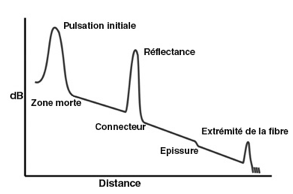
\includegraphics[width=\textwidth - \textwidth / 5]{ressources/r306/00.png}
      \caption{Le signal faiblit naturellement avec la distance. La zone morte correspond à la zone de non visibilité de l'appareil (la lumière étant trop forte pour y dicerner quelque chose, plus on émet fort). Un connecteur (comme une prise) fait joindre verticalement ou horizontalement pour les plus récents deux jartières ("câbles") : la lumière rencontre un obstacle car de l'air est entre et y est réfléchie, ce qui provoque une réflectance et une augmentation du niveau de puissance reçue pour l'appareil. Une épissure est une jonction soudée de deux noyaux de silice.}
      \label{fig:r306-00}
\end{figure}

Ce diagramme a été fait sur une longeur d'onde, mais il pourrait être applicable sur d'autres longueurs d'ondes fréquemment utilisées. Celles-ci sont différenciées selon si elles sont utilisées pour des fibres dites monomode (1310 nm et 1550 nm) à un seul chemin ou multimodes (850 nm et 1300 nm) à chemins multiples. Ces longeurs ont été choisies car l'atténuation y est moins importante pour la lumière. La fibre monomode est souvent préférée aujourd'hui.
\\ \\
Beaucoup d'autres notions ont été abordées : cône d'acceptance, fibres multimode à gradient d'indice, protocole GPON...

\section{Apprentissages pratiques}

Nous avons pu manipuler lors des séances de travaux pratiques des réflectomètres et des fibres optiques afin de monter et caractériser nos premières liaisons.
\\ \\
Un réflectomètre est un appareil de mesure permettant de caractériser le passage de la lumière dans une fibre optique pour s'assurer de son intégrité. Nous avons revu avec eux la différence entre zone morte et zone aveugle, les atténuations générées par les manipulations humaines et tout l'importance de changer la longueur d'onde envoyée selon la distance que l'on souhaite observer.

\begin{figure}[H]
      \centering
      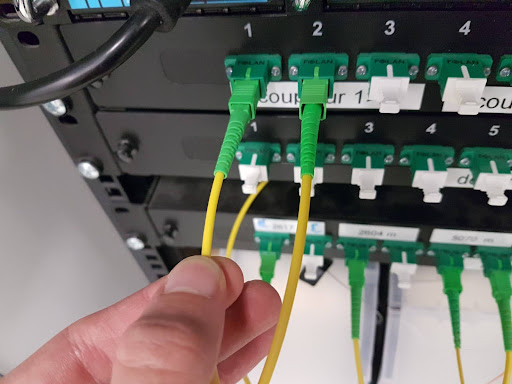
\includegraphics[width=\textwidth - \textwidth / 5]{ressources/r306/01.jpg}
      \caption{Utilisation de l'infrastructure de la salle pour simuler nos premières fibres.}
      \label{fig:r306-01}
\end{figure}

Nous avons aussi vu la technologie WDM. Contrairement aux fibres monomodes qui transportent une longeur d'onde mais en empruntant plusieurs chemins; WDM permet de faire circuler plusieurs longeurs d'ondes, donc plusieurs informations, dans le même support. Cette technologie est extrêmement utilisé dans les coeurs de réseaux opérateur.

\begin{figure}[H]
      \centering
      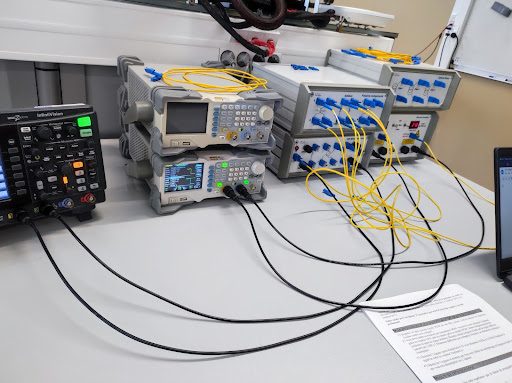
\includegraphics[width=\textwidth - \textwidth / 5]{ressources/r306/00.jpg}
      \caption{Mise en place et caractérisation d'une structure WDM en travail pratique.}
      \label{fig:r306-02}
\end{figure}